%%%%%%%%%%%%%%%%%%%%%%%%%%%%%%%%%%%%%%%%%

%\title{Title page with logo}
%----------------------------------------------------------------------------------------
%	PACKAGES AND OTHER DOCUMENT CONFIGURATIONS
%----------------------------------------------------------------------------------------

\documentclass[12pt]{article}
\usepackage[portuguese]{babel}
\usepackage[utf8x]{inputenc}
\usepackage{amsmath}
\usepackage{graphicx}
\usepackage{natbib}
\usepackage{cite} 
\usepackage{float}
\usepackage{calrsfs}
\usepackage[a4paper,left=2.5cm,right=2.5cm,top=2.5cm, bottom=2.5cm]{geometry}


\begin{document}

\begin{titlepage}

\newcommand{\HRule}{\rule{\linewidth}{0.5mm}} % Defines a new command for the horizontal lines, change thickness here

\center % Center everything on the page
 
%----------------------------------------------------------------------------------------
%	HEADING SECTIONS
%----------------------------------------------------------------------------------------

\textsc{\LARGE Universidade Federal de Alagoas}\\[1.5cm] % Name of your university/college
\textsc{\Large Instituto de Computação (IC)}\\[0.5cm] % Major heading such as course name
\textsc{\large Laboratório de Computação Científica e Análise Numérica (LaCCAN)}\\[3.5cm] % Minor heading such as course title

%----------------------------------------------------------------------------------------
%	TITLE SECTION
%----------------------------------------------------------------------------------------

\HRule \\[0.4cm]
{ \LARGE \bfseries Estimadores dos parâmetros para a Distribuição $G_I^0$}\\[0.4cm] 
\HRule \\[2.5cm]
 
%----------------------------------------------------------------------------------------
%	AUTHOR SECTION
%----------------------------------------------------------------------------------------

\begin{minipage}{0.4\textwidth}
\begin{flushleft} \large
\emph{Autor:}\\
Marcos G. S. do Nascimento % Your name
\end{flushleft}
\end{minipage}
~
\begin{minipage}{0.4\textwidth}
\begin{flushright} \large
\emph{Orientador:} \\
Alejandro C. Frery  % Supervisor's Name
\end{flushright}
\end{minipage}\\[8cm]

% If you don't want a supervisor, uncomment the two lines below and remove the section above
%\Large \emph{Author:}\\
%John \textsc{Smith}\\[3cm] % Your name

%----------------------------------------------------------------------------------------
%	DATE SECTION
%----------------------------------------------------------------------------------------

{\large 24/10/2018}\\[2cm] % Date, change the \today to a set date if you want to be precise

%----------------------------------------------------------------------------------------
%	LOGO SECTION
%----------------------------------------------------------------------------------------

% \includegraphics{logo.png}\\[1cm] % Include a department/university logo - this will require the graphicx package
 
%----------------------------------------------------------------------------------------

\vfill % Fill the rest of the page with whitespace

\end{titlepage}


\section{Introdução}
%%% ACF Evite usar "\\" e qualquer outra formatação fixa

Conforme \citet{FreryMinute2004}, o sensoriamento remoto por microondas pode ser usado para obter informações sobre cenas inacessíveis e/ou não observáveis. A superfície de Vênus, remota e invisível devido à constante cobertura de nuvens, foi mapeada usando sensores de radar. Sensores semelhantes, ou seja, radares de abertura sintética (SARs) são usados para monitorar regiões terrestres inacessíveis, como a Amazônia, os polos e assim por diante. Imagens de ultra-som B são empregadas para diagnosticar sem invadir o corpo. Imagens de sonar são usadas para mapear o fundo do mar, lagos e rios profundos ou escuros, e a iluminação a laser pode ser usada para rastrear perfis de entidades microscópicas.

Essas imagens são formadas por sensores ativos (já que carregam sua própria fonte de iluminação) que enviam e recuperam sinais cuja fase é registrada, ou seja, são  obtidas com radiação coerente. As imagens são formadas detectando o eco do alvo (backscatter) e, nesse processo, um ruído é introduzido devido a fenômenos de interferência. A esse ruído, damos o nome de $speckle$. As propriedades do ruído ($speckle$) são bem descritas pelo modelo multiplicativo, uma estrutura estatística a partir da qual derivam várias distribuições importantes. Entre essas distribuições, uma é considerada o Modelo Universal para dados ruidosos, a saber, a lei $G^{0}$. Esse relatório aborda dados em intensidade, então a distribuição $G_I^0$ será utilizada na estimação dos parâmetros.

\section{O Modelo Universal (Lei $G^{0}$)}

A modelagem estatística dos dados é essencial para interpretar imagens SAR. O artigo de pesquisa de \citet{Gao2010StatisticalMO} discute em detalhes vários modelos estatísticos para esse tipo de dado.
%%% ACF Por que o sobrenome GAO aparece em maiúsculas?

%%% ACF Use modo matemático
Segundo \citet{Mejail2002}, dentre os modelos estatísticos disponíveis, o modelo multiplicativo baseia-se no pressuposto de que o campo aleatório observado (retorno) $Z$ é o resultado do produto de dois campos aleatórios independentes e não observados: $X$ e $Y$. O campo aleatório $X$ modela o retroespalhamento (\textit{backscatter})  do terreno e, portanto, depende apenas do tipo de área a que cada pixel pertence. O campo aleatório $Y$ leva em consideração que as imagens SAR são o resultado de um sistema de geração de imagens coerente que produz o conhecido fenômeno chamado ruído $speckle$, e que elas são geradas pela média de $n$ imagens (teoricamente independentes) - $looks$ - para reduzir o efeito do \textit{speckle}.

Conforme proposto e avaliado em \citet{Clutter1997}, as distribuições $G^0$ podem ser utilizadas com sucesso para descrever os dados contaminados pelo ruído (\textit{speckle}). Dessa forma, os dados ruidosos foram descritos no modelo multiplicativo usando a família $G$ de distribuições que é capaz de descrever áreas extremamente  melhor que a distribuição $K$. Foi demonstrado que essa classe de distribuições é capaz de caracterizar um grande número de alvos em imagens de SAR monopolarizadas, merecendo a denominação de “Modelo Universal”. 

\subsection{Introdução ao Modelo $G_I^0$}

Segundo \citet{FreryStochasticDistances2015}, o modelo $G_I^0$ é indexado por três parâmetros: o número de $Looks$ ($L$) que pode ser estimado em toda a imagem, um parâmetro de escala ($\gamma$) e o parâmetro de rugosidade ou textura ($\alpha$). Este último está intimamente relacionado ao número de $backscatters$ elementares em cada pixel, uma das razões para receber atenção na literatura. Embora haja esforços em fornecer estimativas aprimoradas e robustas para tal quantidade, sua estimativa confiável ainda apresenta problemas numéricos na prática. Vale ressaltar ainda que o número de $Looks$ consiste em um parâmetro que pode ser controlado no processo de geração de imagens e, portanto, será considerado conhecido. Este parâmetro está relacionado à relação sinal-ruído e à precisão espacial da imagem.

Como discutido anteriormente sobre o Modelo Multiplicativo, o retorno em imagens SAR monopolarizadas pode ser modelado como o produto de duas variáveis aleatórias independentes, uma correspondendo ao $backscatter$ $X$ e a outra ao $speckle$ $Y$. Desta maneira, $Z = XY$ representa o retorno em cada pixel sob o modelo multiplicativo. 

Para dados monopolarizados e no caso da distribuição $G_I^0$, o $speckle$ é modelado como uma variável aleatória $Gama$ ($\Gamma$), com média unitária e parâmetro de forma $L \geq 1$, que corresponde ao número de $Looks$, ou seja, o $speckle$ é modelado seguindo a distribuição dada por $\Gamma(L,1)$. O \textit{backscatter}, por sua vez, é considerado obedecendo a uma recíproca da lei $Gama$, isto é, $\Gamma^{-1}(\alpha,\gamma)$. 

Temos que, se $Z \sim G_I^0(\alpha, \gamma, L)$, então sua função de densidade de probabilidade é dada por
%%% ACF Não deixe espaço antes de elementos que fazem parte do parágrafo. Repare no uso de \text
\begin{equation}
    f_Z(z; \alpha, \gamma, \textit{L})= \frac{L^L\Gamma(L-\alpha)z^{L-1}}{\gamma^\alpha\Gamma(-\alpha)\Gamma(L)(\gamma + zL)^{L-\alpha}} \label{eq:fdpGI0}
\end{equation}
onde $-\alpha, \gamma, z > 0$ e $L \geq 1$. $\Gamma$, neste caso, representa a função $gama$. Os parâmetros $\alpha$ e $\gamma$ nesta função de densidade são os parâmetros desconhecidos.

Por sua vez, os momentos de ordem $r$ ($r$-order moments) são dados por
\begin{equation}
    E(Z^r) = \left (\frac{\gamma}{L}\right )^{r}\frac{\Gamma(-\alpha-r)\Gamma(L+r)}{\Gamma(-\alpha)\Gamma(L)} \label{eq:moments}
\end{equation}
fornecidos dessa forma se $\alpha < -r$, e são infinitos, caso contrário.

No processo de estimação, podemos fazer simplificações para reduzir a complexidade dos cálculos e tornar os resultados comparáveis. Para isso, por exemplo, podemos escolher o parâmetro de escala ($\gamma$) de modo que se tenha $E(Z) = 1$, que é dado por $\gamma* = -\alpha - 1$. 

Uma característica crucial da distribuição caracterizada por \eqref{eq:fdpGI0} é que seus parâmetros são interpretáveis: $\gamma$ é um parâmetro de escala e o número de $Looks$ é conhecido antecipadamente ou é estimado para a imagem inteira usando alvos estendidos (amostras muito grandes). Uma das características mais importantes da distribuição $G_I^0$ é a interpretação de seu parâmetro $\alpha$ que está relacionado com a rugosidade do alvo. Valores próximos de $0$ (tipicamente acima de $-3$) sugerem alvos extremamente texturizados, como zonas urbanas. Em situações intermediárias, à medida que o valor diminui, isso indica regiões com textura moderada (geralmente $\alpha \in  [−6, −3]$), tipicamente áreas irregulares, como zonas florestais. Alvos sem textura, geralmente produzem $\alpha \in (−\infty, −6)$ como é o caso de regiões lisas, por exemplo, pastagem, culturas e campos queimados. Esta é a razão pela qual a precisão na estimativa de $\alpha$ é tão importante.

A figura a seguir apresenta as curvas de densidade da distribuição $G_I^0$ para determinados parâmetros.
% GI0 Densities
\begin{figure}[H]
     \centering
     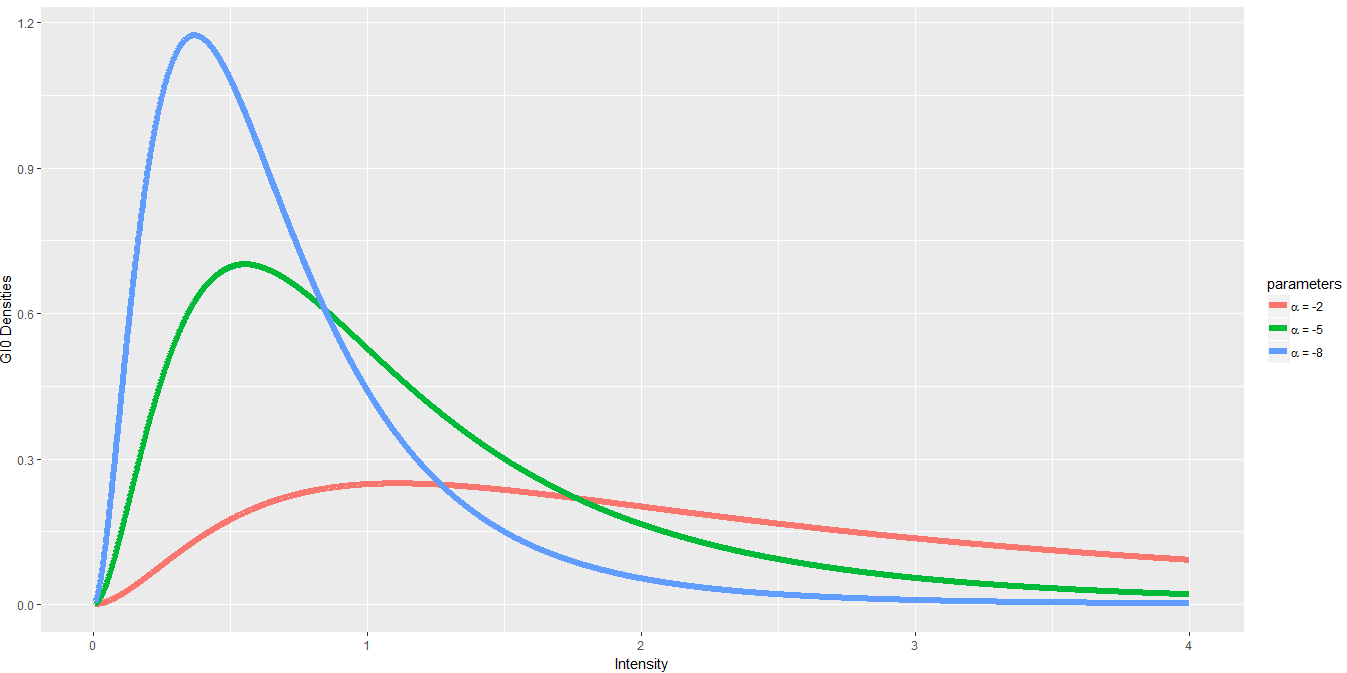
\includegraphics[scale=0.5]{GI0Densities.png}
     \caption{Densidades da distribuição $G_I^0(\alpha, 5, 3)$, com $\alpha \in \left \{  -8, -5, -2 \right \}$}
     \label{graf_1}
\end{figure}

Vale reforçar que Sistemas que empregam iluminação coerente são usados para explorar regiões inacessíveis e/ou inobserváveis (a superfície de Vênus, o interior do corpo humano, o fundo do mar, áreas sob nebulosidade, etc.). É, portanto, de suma importância poder fazer inferências confiáveis sobre o tipo de alvo em análise, uma vez que informações visuais raramente estão disponíveis.


\subsection{Estimação por Máxima Verossimilhança}

As técnicas usuais de inferência incluem métodos baseados no princípio de analogia, sendo os estimadores estatísticos de ordem e momento os mais populares desta classe, e no princípio de Máxima Verossimilhança (MV). Estimadores de momentos são favorecidos em aplicações, já que são fáceis de derivar e são, geralmente, computacionalmente atraentes. Os estimadores MV são amplamente utilizados, uma vez que possuem propriedades ótimas bem conhecidas, como consistência, eficiência e normalidade assintótica, entre outras. Esses estimadores foram utilizados para a análise de imagens de SAR sob o modelo $K$ no trabalho de \citet{KMaxVer_Joughin}.

Dado uma amostra $Z = (Z_1, Z_2, \dots, Z_N)$ e assumindo que essas observações são resultados de variáveis aleatórias independentes e identicamente distribuídas que seguem a distribuição $D(\theta)$, com $\theta \in \Theta$, um estimador MV para $\theta$ é dado por
%%% ACF Use \arg\max
\begin{equation}
    \widehat{\theta} = \arg\max L(\theta; z) \quad \text{para} \quad \theta \in \Theta, \label{eq:mv}
\end{equation}
em que $L$ é a função de verossimilhança da amostra $Z$ sob o parâmetro $\theta$. Podemos utilizar as propriedades logarítmicas para simplificar os cálculos, aplicando o logaritmo natural, visto que o ponto que produz o máximo da função não varia, independentemente de aplicar o logaritmo. Além disso, sob várias condições é equivalente e muitas vezes mais fácil trabalhar com a função log-verossimilhança reduzida $l(\theta; Z)$, onde todos os termos que não dependem de $\theta$ são ignorados.

Embora a maximização direta de \eqref{eq:mv} seja possível (seja analiticamente ou usando ferramentas numéricas) e desejável, muitas vezes encontramos estimadores de MV resolvendo o sistema de equações (geralmente não-lineares) dado por
\begin{equation}
    \nabla l(\widehat{\theta}) = 0 \label{eq:gradient} 
\end{equation}
onde, neste caso, $\nabla$ denota o gradiente. Segundo \citet{FreryMinute2004}, a escolha entre resolver \eqref{eq:mv} ou \eqref{eq:gradient} depende muito de questões computacionais: disponibilidade de algoritmos confiáveis, esforço computacional necessário para implementar e/ou obter a solução e assim por diante. Essas equações, em geral, não têm solução explícita.

Para a construção dos estimadores de Máxima Verossimilhança para o modelo $G_I^0$, considere $Z = (Z_1, Z_2, \dots, Z_N)$ uma amostra aleatória de $N$ variáveis, independentes e igualmente distribuídas, que seguem essa distribuição. Os parâmetros $\alpha$ e $\gamma$ são desconhecidos, enquanto que o parâmetro $Looks$ é conhecido. Nesse caso, a função de verossimilhança é $L((\alpha, \gamma); Z) = \prod_{i=1}^{N} f_Z(Z_i)$, onde $f_Z$ é a função densidade de probabilidade definida anteriormente em \eqref{eq:fdpGI0}. 

Assim, a função de log-verossimilhança ($\log L$) é escrita como
\begin{equation}
    \log L((\alpha, \gamma); Z) = N\log \frac{L^{L}\Gamma(L-\alpha)}{\gamma^{\alpha}\Gamma(-\alpha)\Gamma(L)} +  (L-1)\sum_{i=1}^{N}\log Z_i - (L-\alpha)\sum_{i=1}^{N}\log (\gamma + Z_iL) \label{eq:logVer}
\end{equation}

A partir da função acima, podemos escrever a função de log-verossimilhança reduzida ($l$), excluindo os termos que não dependem de $\alpha$ e $\gamma$
\begin{equation}
    l((\alpha, \gamma); Z) = N\log\Gamma(L-\alpha) - N\alpha \log\gamma - N\log\Gamma(-\alpha) - (L-\alpha)\sum_{i=1}^{N}\log(\gamma +Z_iL) \label{eq:logVerRed}
\end{equation}

O sistema de equações representado em \eqref{eq:gradient} é, em nosso caso, dado por
\begin{equation}
  \frac{\partial l}{\partial \widehat{\alpha}} = N[\Psi(-\widehat{\alpha}) - \Psi(L-\widehat{\alpha})] + \sum_{i=1}^{N}\log\frac{\widehat{\gamma} + Z_iL}{\widehat{\gamma}} = 0
\end{equation}
\begin{equation}
   \frac{\partial l}{\partial \widehat{\gamma}} = -N\frac{\widehat{\alpha}}{\widehat{\gamma}} - (L - \widehat{\alpha})\sum_{i=1}^{N}(\widehat{\gamma} + Z_iL)^{-1} = 0
\end{equation}
em que $\Psi(\tau) = \frac{\textit{d}log\Gamma(\tau)}{\textit{d}\tau}$ é a função $Digama$. Resolvendo esse sistema de equações obtemos os estimadores para os parâmetros $\alpha$ e $\gamma$ da distribuição $G_I^0$, denotados por $\widehat{\alpha}$ e $\widehat{\gamma}$. Em geral, nenhuma solução explícita para este sistema está disponível e, portanto, rotinas numéricas têm que ser usadas.

Assumindo a simplificação feita para o parâmetro de escala ($\gamma* = -\alpha - 1$), temos que o estimador de Máxima Verossimilhança para o parâmetro $\alpha$, chamado $\widehat{\alpha}$, é dado pela solução da seguinte equação não linear:
\begin{eqnarray}
    \Psi(-\widehat{\alpha}) - \Psi(L-\widehat{\alpha}) - \log(-\widehat{\alpha}-1) - \frac{\widehat{\alpha}}{\widehat{\alpha}+1} + \nonumber \\ \frac{1}{N}\sum_{i=1}^{N}\log(-\widehat{\alpha} - 1 + LZ_i) - \left ( \frac{\widehat{\alpha}-L}{N} \right )\sum_{i=1}^{N}(-\widehat{\alpha} - 1 + LZ_i)^{-1} & = & 0
\end{eqnarray}

\subsection{Estimação pelo Método dos Momentos}

Uma outra forma de encontrar estimadores de parâmetros populacionais, como a média e a variância por exemplo, é através do método dos momentos. Este método é baseado na comparação dos momentos teóricos com os momentos amostrais das variáveis aleatórias envolvidas, a partir de uma amostra de $N$ observações.

Seja $Z$ uma variável aleatória contínua com função densidade de probabilidade $f_Z(z)$, os momentos teóricos são dados por $m_j = \int x^jf_Z(z)dz$. Os momentos amostrais, por sua vez, são definidos como $\widehat{m_j} = N^{-1}\sum_{i=1}^{N}z_i^j$. O índice $\textit{j}$ representa a ordem do momento. Após calcular os momentos teóricos e amostrais, o processo de inferência é simples e consiste em comparar os momentos amostrais, $\widehat{m_j}$, com os correspondentes momentos teóricos, $m_j$, até se ter tantas equações quantos forem os parâmetros a serem estimados. De posse do sistema de equações, basta resolver e calcular os estimadores para os parâmetros.

Para estimar os parâmetros $\alpha$ e $\gamma$ da distribuição $G_I^0(\alpha, \gamma, L)$, é necessário estimar dois momentos. Neste relatório, serão utilizados momentos de ordem $\frac{1}{2}$ e $1$, ou seja, $m_{1/2}$ e $m_1$ respectivamente. Esses momentos, de acordo com a equação \eqref{eq:moments}, são dados por
\begin{equation}
    m_{1/2} = \left ( \frac{\gamma}{L}\right )^{1/2} \frac{\Gamma(-\alpha-1/2)\Gamma(L+1/2)}{\Gamma(-\alpha)\Gamma(L)} \quad \text{para} \quad \alpha < -1/2 \label{eq:m12}
\end{equation}
\begin{equation}
    m_{1} = \left ( \frac{\gamma}{L}\right ) \frac{\Gamma(-\alpha-1)\Gamma(L+1)}{\Gamma(-\alpha)\Gamma(L)} \quad \text{para} \quad \alpha < -1 \label{eq:m1}
\end{equation}

Podemos utilizar o momento $\widehat{m}_{1/2}^2$ para auxiliar nos cálculos e utilizar as equações acima \eqref{eq:m12} e \eqref{eq:m1} para determinar o estimador $\widehat{\alpha}$ que pode ser dado como solução da seguinte equação
\begin{equation}
    g(\widehat{\alpha}) - \zeta = 0
\end{equation}
onde 
\begin{equation}
    g(\widehat{\alpha}) = \frac{\Gamma^2(-\widehat{\alpha} - 1/2)}{\Gamma(-\widehat{\alpha})\Gamma(-\widehat{\alpha} - 1)}
\end{equation}
e
\begin{equation}
    \zeta = \frac{\widehat{m}_{1/2}^2\Gamma(L)\Gamma(L+1)}{\widehat{m}_{1}\Gamma^2(L+1/2)}
\end{equation}
Dessa forma, encontrando o valor de $\widehat{\alpha}$ e o substituindo na equação \eqref{eq:m12} ou na equação \eqref{eq:m1}, obtemos o estimador $\widehat{\gamma}$.

Como já mencionado, podemos simplificar o processo de estimação do parâmetro $\gamma$, obtendo-o este de tal forma que o valor esperado $E(Z^r)$ tenha valor unitário e, assim, definimos ele em função do parâmetro $\alpha$. Dessa forma, podemos encontrar $\gamma*$ a partir de \eqref{eq:moments} como a seguir
\begin{equation}
    E(Z^r) = 1 \Rightarrow \left (\frac{\gamma*}{L}\right ) \frac{\Gamma(-\alpha-1)\Gamma(L+1)}{\Gamma(-\alpha)\Gamma(L)} = 1 \Rightarrow \gamma* = L\left ( \frac{\Gamma(-\alpha)\Gamma(L)}{\Gamma(-\alpha-1)\Gamma(L+1)} \right ) 
\end{equation}
onde, fazendo $\Gamma(n) = (n-1)!$, temos
\begin{equation}
    \gamma* = -\alpha - 1
\end{equation}
Estimadores de momentos fracionários foram utilizadas amplamente em \citet{Clutter1997} e, dessa forma, assumindo a simplificação acima e utilizando $r=\frac{1}{2}$  em \eqref{eq:moments} é preciso resolver a equação a seguir para se obter o estimador $\widehat{\alpha}$
\begin{equation}
    \frac{1}{N}\sum_{i=1}^{N}\sqrt{z_i}-\sqrt{\frac{-\widehat{\alpha} - 1}{L}}\frac{\Gamma(-\widehat{\alpha} - \frac{1}{2})}{\Gamma(-\widehat{\alpha})}\frac{\Gamma(L+\frac{1}{2})}{\Gamma(L)} = 0
\end{equation}

\section{Propostas de Implementação dos Estimadores}

Para a implementação dos estimadores foi proposto o uso do pacote \texttt{stats4} que disponibiliza a função \texttt{mle} que pode ser utilizada para se obter os estimadores de Máxima Verossimilhança tanto de distribuições populares, por exemplo, $Normal$, $Gama$ e $t$, quanto de distribuições que não possuem implementação nativa na plataforma \textit{R}.

Foi feita a implementação dos estimadores de MV para o modelo $G_I^0$ utilizando esse pacote. Nessa implementação, utilizou-se dados simulados gerados pelo gerador de variáveis aleatórias $G_I^0$ implementado a partir do Modelo Multiplicativo, onde as variáveis aleatórias são geradas a partir da razão de variáveis aleatórias $Gama$.

Os dados foram gerados seguindo a distribuição $G_I^0(-8, 7, 3)$ com o parâmetro de textura $\alpha$ valendo $-8$, o parâmetro de escala $\gamma$ valendo $7$ e o número de $Looks$ com valor 3. O número de variáveis aleatórias geradas foi $n = 200$.

Como nota-se em \eqref{eq:mv}, a estimação por Máxima Verossimilhança consiste em encontrar o $\arg\max$ da função de Verossimilhança e, com base nessa ideia, estamos diante de um problema de otimização. Um método utilizado para encontrar tais pontos de máximo é fazer como em \eqref{eq:gradient}, calculando as derivadas parciais e igualando a zero. Mas, como alternativa a isso, podemos aplicar diversos otimizadores existentes na literatura e que estão disponíveis para uso na função \textit{mle} do pacote \textit{stats4}.

Dentre os otimizadores disponíveis, temos, talvez o mais utilizado deles, o \emph{BFGS} é um método quasi-Newton (também conhecido como algoritmo variável de métrica), especificamente aquele publicado simultaneamente em 1970 por Broyden, Fletcher, Goldfarb e Shanno. Esse algoritmo usa valores de função e gradientes para construir uma imagem da superfície a ser otimizada. Na simulação feita, foi utilizado o otimizador \emph{L-BFGS-B} é o de \citet{Byrd_1995}, que permite restrições de limite, ou seja, cada variável pode receber um limite inferior e/ou superior. O valor inicial deve satisfazer as restrições. Ou seja, ele consiste de uma modificação de memória limitada do método \emph{BFGS} quasi-Newton e que diminui o espaço de busca dos valores para os estimadores.

Na simulação feita, também foi utilizada o otimizador de \emph{Brent} que é utilizado somente para problemas unidimensionais, neste caso, utilizou-se a simplificação feita de que $\widehat{\gamma}* = -\widehat{\alpha} - 1$ e, fornecemos para o algoritmo somente o parâmetro de textura $\alpha$ para ser otimizado.

Para finalizar, foram feitos testes também com o otimizador \emph{CG} que é um método de gradientes conjugados baseado em \citet{Fletcher64}. Métodos baseados em gradiente conjugado geralmente são mais frágeis que aqueles baseados no método \emph{BFGS}, entretanto, como eles não armazenam uma matriz, podem ter sucesso em problemas de otimização muito maiores e mais complicados. 

Os estimadores para cada um dos 3 otimizadores utilizados estão dispostos na tabela abaixo.
\begin{table}[H]
\centering
\caption{Estimadores MV para os parâmetros de textura($\alpha$) e escala($\gamma$)}
\vspace{0.2cm}
\begin{tabular}{r|r|r|lr}
\hline
Estimadores & L-BFGS-B & CG & Brent \\ 
\hline                               
$\widehat{\alpha}_{MV}$ & -8.229604 & -8.126974 & -8.414278 \\
$\widehat{\gamma}_{MV}$ & 7.324793 & 7.223863 & 7.414278 \\
\end{tabular}
\end{table}

Como pode-se observar, os estimadores calculados utilizando o otimizador \emph{CG} baseado em gradientes conjugados apresentou o menor erro em relação aos demais. Entretanto, foram feitos testes com outros tamanhos de variáveis geradas, $n={500, 800, 1000}$ e, na maioria das vezes, o otimizador baseado em \emph{L-BFGS-B} obtem os melhores resultados.

Para os estimadores de Momentos, as propostas de implementação ainda não estão bem consolidadas e, na verdade, ainda se está averiguando as bibliotecas existentes e como estas poderiam ser aplicadas no contexto da estimação dos parâmetros da $G_I^0$. Algumas bibliotecas foram pesquisadas e estudadas, mas não houveram tantos avanços nessa parte ainda. As bibliotecas \textit{gmm} (Generalized Method of Moments) e \textit{moments} foram instaladas e usadas para pequenos testes e, além dessas, estou analisando outras que possam ser úteis na estimação. Portanto, os trabalhos futuros consistem em direcionar os esforços nesta parte de implementação e análise dos estimadores, com foco tanto nos estimadores de Máxima Verossimilhança quanto nos estimadores de Momentos, ambos discutidos no presente relatório. 

\newpage
\bibliographystyle{agsm}
%\bibliographystyle{unsrt}
\bibliography{../../../Bibliography/references}
%\bibliography{references}


\end{document}